\documentclass[12pt]{article}
\usepackage{geometry} % see geometry.pdf on how to lay out the page. There's lots.
\usepackage{graphicx}
\geometry{a4paper} % or letter or a5paper or ... etc
% \geometry{landscape} % rotated page geometry

% See the ``Article customise'' template for come common customisations

\title{Report on Visualization Project}
\author{Daiqi Linghu, Dunzhu Li, Yiran Ma}
\date{} % delete this line to display the current date


% define argmin
\usepackage{amsmath}
\newcommand{\argmin}{\operatornamewithlimits{argmin}}
\newcommand\norm[1]{\left\lVert#1\right\rVert}

%%% BEGIN DOCUMENT
\begin{document}

\maketitle
%\tableofcontents

% Introduction
\section{Introduction}
In this project, the data we tackle with are the user ratings of the movies, and we aim to create two-dimensional illustrations of the latent factors. The formulation of the problem is:
\begin{equation*}
Y_{M\times N} = U_{K\times M}^{T} V_{K\times N}
\end{equation*}
where M is the number of users, N is the number of movies, Y is the rating matrix, U and V are the latent factors. 

We first solve for U and V using Bias-Stochastic Gradient Descent (BSGD) method, and then, visualize U and V through projection.  

% Algorithm
\section{Algorithm}
\subsection{Optimization}
To solve for the latent factors U and V, we solve the following optimization problem:
\begin{equation*}
\argmin_{U,V,a,b}\frac{\lambda}{2}\left(\norm{U}^2+\norm{V}^2+\norm{a}^2+\norm{b}^2\right)+
\sum_{(i,j)\in S}\left(  Q_{i,j}  \right)^2
\end{equation*}
where $Q_{i,j}=(u_i^T v_j + a_i + b_j +\mu-Y_{i,j})$. Then,

\begin{equation*}
\frac{\partial{J}}{\partial{U_{l}}}=\lambda U_{l}+\sum_{(i,j)\in S}2Q_{i,j}1_{i=l}V_{j}
\end{equation*}

We call the first term in the gradient as ``norm term'', and the second term ``error term''.

$U_{l}$ is updated iteratively through gradient method:
\begin{equation*}
U_{l}^{n+1}=U_{l}^{n}-\eta \frac{\partial{J}}{\partial{U_{l}}}
\end{equation*}

In BSGD, for each iteration, we randomly loop through all the data and update $U_{l}$ with ``error term'' only in the loop, then after the loop, correct $U_{l}$ with ``norm term''. We can do $V_{k}$, $a_{l}$ and $b_{k}$ similarly.

\subsection{Visualization}
We project U and V to 2 dimensions and visualize them. First, we compute SVD of V:
\begin{equation*}
V=A\Sigma B^{T}
\end{equation*}
The first two columns of A correspond to best 2-dimensional projection of movies V.

Then, we project every movie ($V_{1:N}$) and user ($U_{1:M}$) using $A_{1:2}$:
\begin{eqnarray*}
\tilde{V}=A_{1:2}^{T} V \in Re^{2\times N}\\
\tilde{U}=A_{1:2}^{T} U \in Re^{2\times N}
\end{eqnarray*}

\section{Implementation}
\subsection{Find U \& V (BSGD.m)}
To solve the optimization problem with Bias-SGD, we simply divide the data by 5 fold, use 4 folds as training data and 1 fold as test data to find the optimal damping parameter $\lambda$  and number of iteration. The step size $\eta$ is chosen as 1e-2 and is decreased by 10\% for each iteration. From the results shown below (Fig. 1), we choose $\lambda=25$. For $\lambda=25$, the out-of-sample error is still decreasing at the 100th iteration (Fig. 1), however, the improvement is minimal. Therefore, we choose the number of iteration as 100.

\begin{figure}[h!]
  \centering
      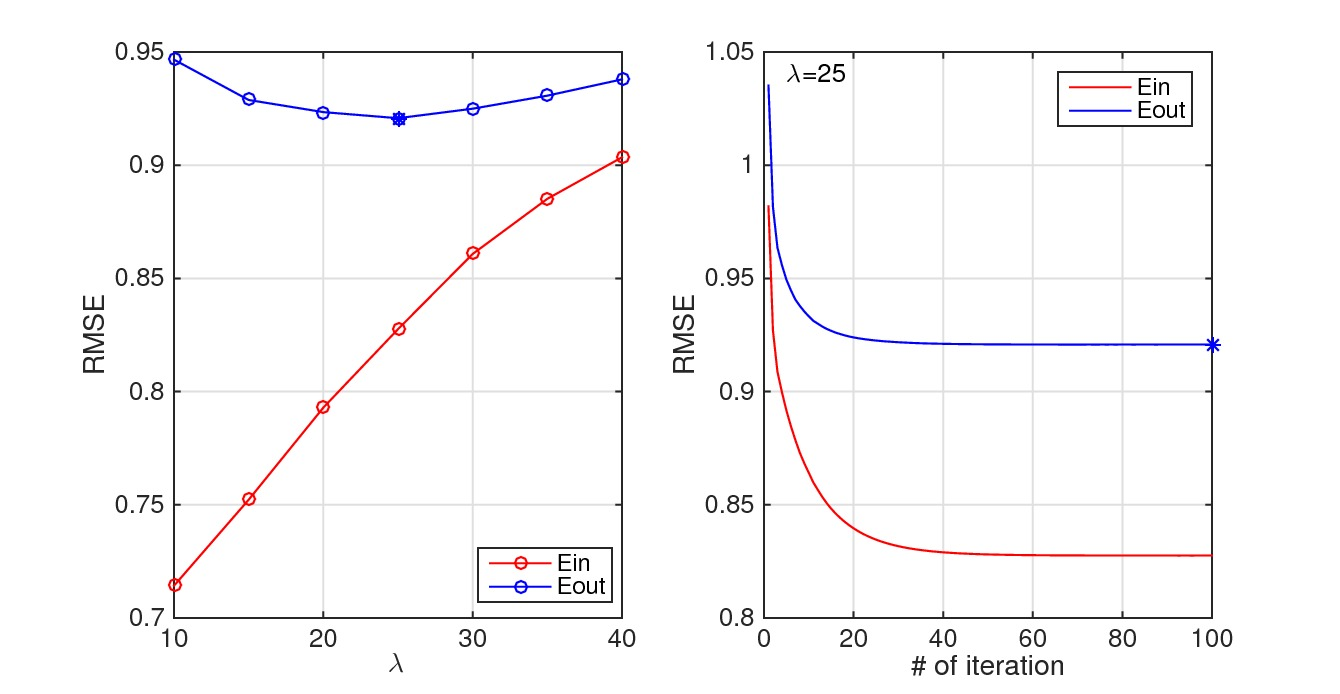
\includegraphics[width=1.0\textwidth]{testparameter}
  \caption{RMS error (RMSE) vs. Parameter. Left: For different $\lambda$, we plot the minimum RMSE in 100 iterations. We see that $\lambda=25$ is the optimum choice. Right: For $\lambda=25$, we plot the RMSEs in 100 iterations. We see that RMSE decays slowly after about 15 iterations. We simply choose the number of iteration as 100 for final run.}
\end{figure}


\subsection{Projection}

\section{Discussions and Conclusions}



\end{document} 